\documentclass{standalone}
\usepackage{tikz}
\usetikzlibrary{patterns, positioning}
\usepackage[sfdefault]{ClearSans} %% option 'sfdefault' activates Clear Sans as the default text font
\usepackage[T1]{fontenc}

\begin{document}
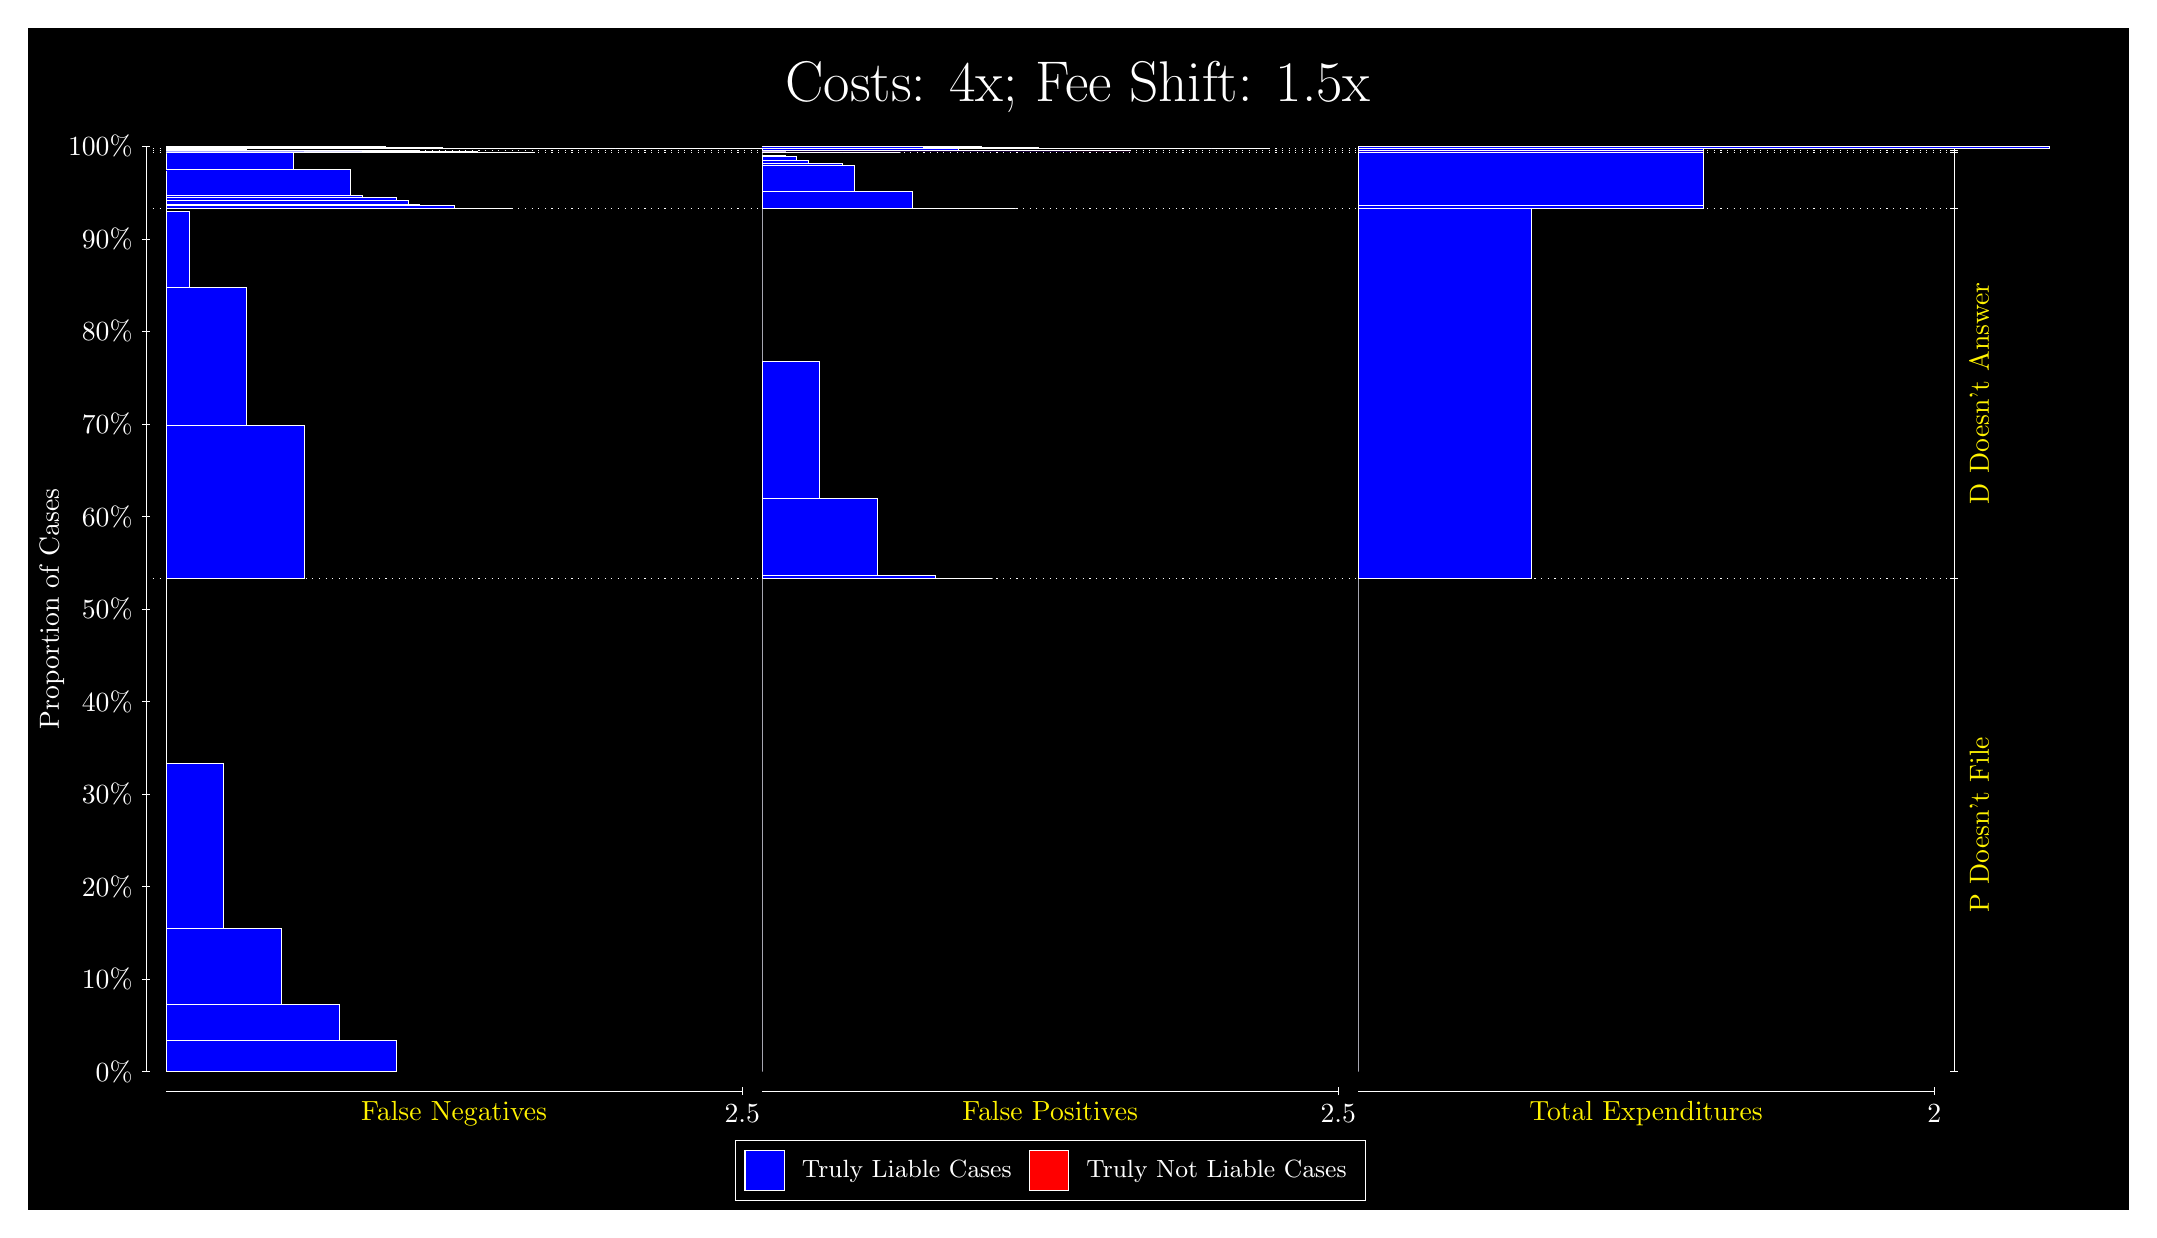
\begin{tikzpicture}
\draw[fill=black] (0,0) rectangle (26.667,15);
\draw[text=white] (0,13.5) rectangle (26.667,15) node[midway] {\huge Costs: 4x; Fee Shift: 1.5x};
\draw[white, very thin] (1.5,1.75) -- (1.5,13.5);
\node[rotate=90, text=white, anchor=center] at (0.3, 7.625) {Proportion of Cases};
\draw[white, very thin] (1.45,1.75) -- (1.55,1.75);
\node[text=white, anchor=east] at (1.45, 1.75) {0\%};
\draw[white, very thin] (1.45,2.925) -- (1.55,2.925);
\node[text=white, anchor=east] at (1.45, 2.925) {10\%};
\draw[white, very thin] (1.45,4.1) -- (1.55,4.1);
\node[text=white, anchor=east] at (1.45, 4.1) {20\%};
\draw[white, very thin] (1.45,5.275) -- (1.55,5.275);
\node[text=white, anchor=east] at (1.45, 5.275) {30\%};
\draw[white, very thin] (1.45,6.45) -- (1.55,6.45);
\node[text=white, anchor=east] at (1.45, 6.45) {40\%};
\draw[white, very thin] (1.45,7.625) -- (1.55,7.625);
\node[text=white, anchor=east] at (1.45, 7.625) {50\%};
\draw[white, very thin] (1.45,8.8) -- (1.55,8.8);
\node[text=white, anchor=east] at (1.45, 8.8) {60\%};
\draw[white, very thin] (1.45,9.975) -- (1.55,9.975);
\node[text=white, anchor=east] at (1.45, 9.975) {70\%};
\draw[white, very thin] (1.45,11.15) -- (1.55,11.15);
\node[text=white, anchor=east] at (1.45, 11.15) {80\%};
\draw[white, very thin] (1.45,12.325) -- (1.55,12.325);
\node[text=white, anchor=east] at (1.45, 12.325) {90\%};
\draw[white, very thin] (1.45,13.5) -- (1.55,13.5);
\node[text=white, anchor=east] at (1.45, 13.5) {100\%};

\draw[white, very thin] (24.457,1.75) -- (24.457,13.5);
\draw[white, very thin] (24.407,1.75) -- (24.507,1.75);
\node[anchor=west] at (24.407, 1.75) {};
\draw[white, very thin] (24.407,8.0162) -- (24.507,8.0162);
\node[anchor=west] at (24.407, 8.0162) {};
\draw[white, very thin] (24.407,12.713) -- (24.507,12.713);
\node[anchor=west] at (24.407, 12.713) {};
\draw[white, very thin] (24.407,13.422) -- (24.507,13.422);
\node[anchor=west] at (24.407, 13.422) {};
\draw[white, very thin] (24.407,13.446) -- (24.507,13.446);
\node[anchor=west] at (24.407, 13.446) {};
\draw[white, very thin] (24.407,13.473) -- (24.507,13.473);
\node[anchor=west] at (24.407, 13.473) {};
\draw[white, very thin] (24.407,13.5) -- (24.507,13.5);
\node[anchor=west] at (24.407, 13.5) {};

\draw[white, very thin, fill=blue] (1.75,1.75) rectangle (4.6775,2.1423);
\draw[white, very thin, fill=blue] (1.75,2.1423) rectangle (3.9457,2.5983);
\draw[white, very thin, fill=blue] (1.75,2.5983) rectangle (3.2138,3.5681);
\draw[white, very thin, fill=blue] (1.75,3.5681) rectangle (2.4819,5.6687);
\draw[white, very thin, fill=red] (1.75,5.6687) rectangle (1.75,5.6687);
\draw[white, very thin, fill=blue] (1.75,5.6687) rectangle (1.75,8.0162);
\draw[white, very thin, fill=blue] (1.75,8.0162) rectangle (3.5065,9.956);
\draw[white, very thin, fill=blue] (1.75,9.956) rectangle (2.7746,11.705);
\draw[white, very thin, fill=blue] (1.75,11.705) rectangle (2.0428,12.68);
\draw[white, very thin, fill=red] (1.75,12.68) rectangle (1.75,12.68);
\draw[white, very thin, fill=blue] (1.75,12.68) rectangle (1.75,12.713);
\draw[white, very thin, fill=blue] (1.75,12.713) rectangle (6.1413,12.713);
\draw[white, very thin, fill=blue] (1.75,12.713) rectangle (5.5558,12.716);
\draw[white, very thin, fill=blue] (1.75,12.716) rectangle (5.4094,12.748);
\draw[white, very thin, fill=blue] (1.75,12.748) rectangle (4.9703,12.762);
\draw[white, very thin, fill=blue] (1.75,12.762) rectangle (4.8239,12.817);
\draw[white, very thin, fill=blue] (1.75,12.817) rectangle (4.6775,12.856);
\draw[white, very thin, fill=blue] (1.75,12.856) rectangle (4.2384,12.876);
\draw[white, very thin, fill=blue] (1.75,12.876) rectangle (4.092,13.203);
\draw[white, very thin, fill=blue] (1.75,13.203) rectangle (3.9457,13.204);
\draw[white, very thin, fill=blue] (1.75,13.204) rectangle (3.5065,13.204);
\draw[white, very thin, fill=blue] (1.75,13.204) rectangle (3.3602,13.419);
\draw[white, very thin, fill=blue] (1.75,13.419) rectangle (3.2138,13.419);
\draw[white, very thin, fill=blue] (1.75,13.419) rectangle (2.7746,13.419);
\draw[white, very thin, fill=blue] (1.75,13.419) rectangle (2.6283,13.422);
\draw[white, very thin, fill=blue] (1.75,13.422) rectangle (2.0428,13.422);
\draw[white, very thin, fill=red] (1.75,13.422) rectangle (1.75,13.422);
\draw[white, very thin, fill=blue] (1.75,13.422) rectangle (6.4341,13.422);
\draw[white, very thin, fill=blue] (1.75,13.422) rectangle (5.7022,13.433);
\draw[white, very thin, fill=blue] (1.75,13.433) rectangle (4.9703,13.446);
\draw[white, very thin, fill=blue] (1.75,13.446) rectangle (4.2384,13.446);
\draw[white, very thin, fill=blue] (1.75,13.446) rectangle (3.5065,13.446);
\draw[white, very thin, fill=red] (1.75,13.446) rectangle (1.75,13.446);
\draw[white, very thin, fill=blue] (1.75,13.446) rectangle (3.5065,13.446);
\draw[white, very thin, fill=blue] (1.75,13.446) rectangle (2.7746,13.462);
\draw[white, very thin, fill=blue] (1.75,13.462) rectangle (2.0428,13.473);
\draw[white, very thin, fill=red] (1.75,13.473) rectangle (1.75,13.473);
\draw[white, very thin, fill=blue] (1.75,13.473) rectangle (1.75,13.473);
\draw[white, very thin, fill=blue] (1.75,13.473) rectangle (13.46,13.473);
\draw[white, very thin, fill=blue] (1.75,13.473) rectangle (12.728,13.473);
\draw[white, very thin, fill=blue] (1.75,13.473) rectangle (11.996,13.473);
\draw[white, very thin, fill=blue] (1.75,13.473) rectangle (11.265,13.477);
\draw[white, very thin, fill=blue] (1.75,13.477) rectangle (10.533,13.477);
\draw[white, very thin, fill=blue] (1.75,13.477) rectangle (9.8008,13.477);
\draw[white, very thin, fill=blue] (1.75,13.477) rectangle (7.4587,13.477);
\draw[white, very thin, fill=blue] (1.75,13.477) rectangle (6.7268,13.477);
\draw[white, very thin, fill=blue] (1.75,13.477) rectangle (5.9949,13.48);
\draw[white, very thin, fill=blue] (1.75,13.48) rectangle (5.2631,13.493);
\draw[white, very thin, fill=blue] (1.75,13.493) rectangle (4.5312,13.5);
\draw[white, very thin, fill=blue] (1.75,13.5) rectangle (3.7993,13.5);
\draw[white, very thin, fill=blue] (1.75,13.5) rectangle (3.0674,13.5);
\draw[white, very thin, fill=blue] (1.75,13.5) rectangle (2.3355,13.5);
\draw[white, very thin, fill=red] (1.75,13.5) rectangle (1.75,13.5);
\draw[white, very thin, fill=red] (9.3189,1.75) rectangle (9.3189,1.75);
\draw[white, very thin, fill=blue] (9.3189,1.75) rectangle (9.3189,8.0162);
\draw[white, very thin, fill=red] (9.3189,8.0162) rectangle (12.246,8.0162);
\draw[white, very thin, fill=blue] (9.3189,8.0162) rectangle (12.246,8.0162);
\draw[white, very thin, fill=blue] (9.3189,8.0162) rectangle (11.515,8.0495);
\draw[white, very thin, fill=blue] (9.3189,8.0495) rectangle (10.783,9.0245);
\draw[white, very thin, fill=blue] (9.3189,9.0245) rectangle (10.051,10.773);
\draw[white, very thin, fill=blue] (9.3189,10.773) rectangle (9.3189,12.713);
\draw[white, very thin, fill=red] (9.3189,12.713) rectangle (12.539,12.713);
\draw[white, very thin, fill=blue] (9.3189,12.713) rectangle (12.539,12.713);
\draw[white, very thin, fill=red] (9.3189,12.713) rectangle (11.954,12.713);
\draw[white, very thin, fill=blue] (9.3189,12.713) rectangle (11.954,12.716);
\draw[white, very thin, fill=blue] (9.3189,12.716) rectangle (11.807,12.716);
\draw[white, very thin, fill=red] (9.3189,12.716) rectangle (11.368,12.716);
\draw[white, very thin, fill=blue] (9.3189,12.716) rectangle (11.368,12.716);
\draw[white, very thin, fill=blue] (9.3189,12.716) rectangle (11.222,12.931);
\draw[white, very thin, fill=blue] (9.3189,12.931) rectangle (11.075,12.931);
\draw[white, very thin, fill=blue] (9.3189,12.931) rectangle (10.636,12.932);
\draw[white, very thin, fill=blue] (9.3189,12.932) rectangle (10.49,13.259);
\draw[white, very thin, fill=blue] (9.3189,13.259) rectangle (10.344,13.279);
\draw[white, very thin, fill=blue] (9.3189,13.279) rectangle (9.9044,13.318);
\draw[white, very thin, fill=blue] (9.3189,13.318) rectangle (9.758,13.373);
\draw[white, very thin, fill=blue] (9.3189,13.373) rectangle (9.6116,13.388);
\draw[white, very thin, fill=blue] (9.3189,13.388) rectangle (9.3189,13.422);
\draw[white, very thin, fill=red] (9.3189,13.422) rectangle (11.075,13.422);
\draw[white, very thin, fill=blue] (9.3189,13.422) rectangle (11.075,13.422);
\draw[white, very thin, fill=blue] (9.3189,13.422) rectangle (10.344,13.422);
\draw[white, very thin, fill=blue] (9.3189,13.422) rectangle (9.6116,13.435);
\draw[white, very thin, fill=blue] (9.3189,13.435) rectangle (9.3189,13.446);
\draw[white, very thin, fill=red] (9.3189,13.446) rectangle (14.003,13.446);
\draw[white, very thin, fill=blue] (9.3189,13.446) rectangle (14.003,13.446);
\draw[white, very thin, fill=blue] (9.3189,13.446) rectangle (13.271,13.446);
\draw[white, very thin, fill=blue] (9.3189,13.446) rectangle (12.539,13.456);
\draw[white, very thin, fill=blue] (9.3189,13.456) rectangle (11.807,13.472);
\draw[white, very thin, fill=blue] (9.3189,13.472) rectangle (11.075,13.473);
\draw[white, very thin, fill=red] (9.3189,13.473) rectangle (15.759,13.473);
\draw[white, very thin, fill=blue] (9.3189,13.473) rectangle (15.759,13.473);
\draw[white, very thin, fill=blue] (9.3189,13.473) rectangle (15.028,13.473);
\draw[white, very thin, fill=red] (9.3189,13.473) rectangle (15.028,13.473);
\draw[white, very thin, fill=blue] (9.3189,13.473) rectangle (15.028,13.473);
\draw[white, very thin, fill=blue] (9.3189,13.473) rectangle (14.296,13.473);
\draw[white, very thin, fill=red] (9.3189,13.473) rectangle (14.296,13.473);
\draw[white, very thin, fill=blue] (9.3189,13.473) rectangle (14.296,13.473);
\draw[white, very thin, fill=blue] (9.3189,13.473) rectangle (13.564,13.475);
\draw[white, very thin, fill=red] (9.3189,13.475) rectangle (13.564,13.475);
\draw[white, very thin, fill=blue] (9.3189,13.475) rectangle (13.564,13.479);
\draw[white, very thin, fill=blue] (9.3189,13.479) rectangle (12.832,13.48);
\draw[white, very thin, fill=blue] (9.3189,13.48) rectangle (12.832,13.493);
\draw[white, very thin, fill=blue] (9.3189,13.493) rectangle (12.1,13.495);
\draw[white, very thin, fill=blue] (9.3189,13.495) rectangle (11.368,13.496);
\draw[white, very thin, fill=blue] (9.3189,13.496) rectangle (10.636,13.496);
\draw[white, very thin, fill=red] (9.3189,13.496) rectangle (9.3189,13.496);
\draw[white, very thin, fill=blue] (9.3189,13.496) rectangle (9.3189,13.5);
\draw[white, very thin, fill=red] (16.888,1.75) rectangle (16.888,1.75);
\draw[white, very thin, fill=blue] (16.888,1.75) rectangle (16.888,8.0162);
\draw[white, very thin, fill=red] (16.888,8.0162) rectangle (19.083,8.0162);
\draw[white, very thin, fill=blue] (16.888,8.0162) rectangle (19.083,12.713);
\draw[white, very thin, fill=red] (16.888,12.713) rectangle (21.279,12.713);
\draw[white, very thin, fill=blue] (16.888,12.713) rectangle (21.279,12.749);
\draw[white, very thin, fill=red] (16.888,12.749) rectangle (21.279,12.749);
\draw[white, very thin, fill=blue] (16.888,12.749) rectangle (21.279,13.422);
\draw[white, very thin, fill=red] (16.888,13.422) rectangle (21.279,13.422);
\draw[white, very thin, fill=blue] (16.888,13.422) rectangle (21.279,13.446);
\draw[white, very thin, fill=red] (16.888,13.446) rectangle (21.279,13.446);
\draw[white, very thin, fill=blue] (16.888,13.446) rectangle (21.279,13.473);
\draw[white, very thin, fill=red] (16.888,13.473) rectangle (25.67,13.473);
\draw[white, very thin, fill=blue] (16.888,13.473) rectangle (25.67,13.48);
\draw[white, very thin, fill=red] (16.888,13.48) rectangle (25.67,13.48);
\draw[white, very thin, fill=blue] (16.888,13.48) rectangle (25.67,13.5);
\draw[white, dotted] (1.5,8.0162) -- (24.457,8.0162);
\draw[white, dotted] (1.5,12.713) -- (24.457,12.713);
\draw[white, dotted] (1.5,13.422) -- (24.457,13.422);
\draw[white, dotted] (1.5,13.446) -- (24.457,13.446);
\draw[white, dotted] (1.5,13.473) -- (24.457,13.473);
\draw[white, very thin] (1.75,1.5) -- (9.0689,1.5);
\node[text=yellow, anchor=north] at (5.4094, 1.5) {False Negatives};
\draw[white, very thin] (9.0689,1.45) -- (9.0689,1.55);
\node[text=white, anchor=north] at (9.0689, 1.45) {2.5};

\draw[white, very thin] (9.3189,1.5) -- (16.638,1.5);
\node[text=yellow, anchor=north] at (12.978, 1.5) {False Positives};
\draw[white, very thin] (16.638,1.45) -- (16.638,1.55);
\node[text=white, anchor=north] at (16.638, 1.45) {2.5};

\draw[white, very thin] (16.888,1.5) -- (24.207,1.5);
\node[text=yellow, anchor=north] at (20.547, 1.5) {Total Expenditures};
\draw[white, very thin] (24.207,1.45) -- (24.207,1.55);
\node[text=white, anchor=north] at (24.207, 1.45) {2};

\node[text=yellow, centered, rotate=90] at (24.777, 4.8831) {P Doesn't File};
\node[text=yellow, centered, rotate=90] at (24.777, 10.365) {D Doesn't Answer};





\draw (12.978300999999998,1.5) node[draw=none] (baseCoordinate) {};
\begin{scope}[align=center]
        \matrix[scale=0.5, draw=white, below=0.5cm of baseCoordinate, nodes={draw}, column sep=0.1cm]{
            \node[rectangle, draw, minimum width=0.5cm, minimum height=0.5cm, fill=blue] {}; &
            \node[draw=none, font=\small, text=white] (B) {Truly Liable Cases}; &
            \node[rectangle, draw, minimum width=0.5cm, minimum height=0.5cm, fill=red] {}; &
            \node[draw=none, font=\small, text=white] (B) {Truly Not Liable Cases}; \\
            };
\end{scope}

\end{tikzpicture}
\end{document}